\section{碱和盐的性质}\label{sec:xssy-sy8}

\begin{shiyanmudi}
    巩固和加深对碱和盐的性质的认识。
\end{shiyanmudi}


\begin{shiyanyongpin}
    试管、pH 试纸、玻璃管、烧杯、玻璃棒、胶头滴管、蒸发皿、酒精灯、铁架台(带铁圈)、药匙。

    氢氧化钠稀溶液、石灰水、稀氨水、石蕊试液、酚酞试液、稀盐酸、稀硝酸、硫酸铜溶液、氯化铁溶液、
    硝酸铅溶液、锌粒、铜片、硫酸钠溶掖、硫酸铵溶液、碳酸钠溶液、氯化钡溶液、氯化钠溶液、硝酸银溶液。
\end{shiyanyongpin}


\begin{shiyanbuzhou}
    1. 碱对指示剂的作用

    (1) 在三个试管里分别倒入氢氧化钠稀溶液、石灰水、稀氨水各 2 毫升,观察它们的颜色,并闻气味。
    用 pH 试纸分别试验这三种溶液,观察颜色的变化,跟比色卡对比,测出这三种碱溶液的 pH 值。

    (2) 在上面三个试管里各滴入 1—2 滴石蕊试液,观察颜色的变化。

    (3) 用酚酞试液试验上面三种溶液。想一想应该怎样操作?并观察颜色的变化。

    2. 碱跟酸性氧化物的反应

    在试管里注入 5 毫升澄清的石灰水,通过一根洁净的玻璃管,用嘴向石灰水里不断地吹气,有什么现象发生?写出反应的化学方程式。

    3. 碱跟酸的反应 —— 中和反应

    (1) 往小烧怀里倒入 5 毫升氢氧化钠稀溶液,再滴入 1—2 滴酚酞试液,有什么现象发生? 然后,一面用玻璃棒不停地搅拌溶液,
    一面用胶头滴管逐滴滴入稀盐酸,一直滴到溶液颜色刚刚变成无色为止。这时,中和反应就完成了。

    (2) 把中和后的溶液的一半倒在蒸发皿里,加热蒸发皿,使溶液蒸发到出现晶体为止。这种晶体是什么?写出反应的化学方程式。

    4. 碱跟盐的反应

    在两个试管里分别倒入 2 毫升硫酸铜溶液和氯化铁溶液。然后,各滴入几滴氢氧化钠溶液,有什么现象发生?写出反应的化学方程式。

    5. 盐跟金属的反应

    在一盛有硫酸铜溶液的试管里,加入锌粒。在另一盛有硝酸铅溶液的试管里,加入铜片。观察发生的现象。写出反应的化学方程式。

    6. 盐跟盐的反应

    (1) 在盛有硫酸钠溶液、硫酸铵溶液和碳酸钠溶液的三个试管里,各滴入氯化钡溶液,有什么现象发生?再各加入少量稀硝酸,又有什么现象发生?写出反应的化学方程式。

    (2) 在盛有氯化钠溶液的试管里,滴入硝酸银溶液,有什么现象发生? 再加入少量稀硝酸,又有什么现象发生?写出反应的化学方程式。
\end{shiyanbuzhou}


\begin{wentihetaolun}
    1. 用什么方法可以鉴别硫酸盐?简述操作步骤和可能发生的现象。

    2. 用盐酸和氢氧化钠做中和反应实验时:

    (1) 为什么要用指示剂?

    (2) 为什么要用滴管逐滴地把盐酸加入碱溶液里?

    (3) 在滴加盐酸的同时,为什么要用玻璃棒不断地搅拌溶液?

    3. 分别指出下列各图中的错误,并分别叙述正确的操作方法。

    \begin{figure}[htbp]
        \centering
        \begin{minipage}[b]{5cm}
            \centering
            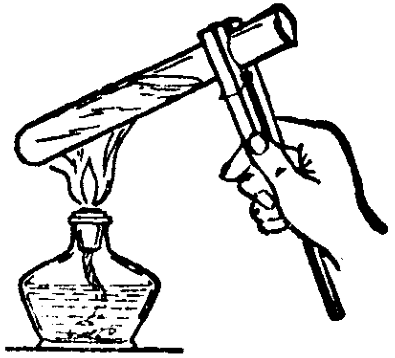
\includegraphics[width=4cm]{../pic/czhx1-xssy-25}
            \caption{\begin{minipage}[t]{4cm}
                用试管夹夹住\\
                试管进行加热
            \end{minipage}}\label{fig:xssy-25}
        \end{minipage}
        \qquad
        \begin{minipage}[b]{3cm}
            \centering
            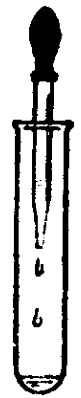
\includegraphics[width=1cm]{../pic/czhx1-xssy-26}
            \caption{\begin{minipage}[t]{2cm}
                用滴管滴\\
                加液体
            \end{minipage}}\label{fig:xssy-26}
        \end{minipage}
        \qquad
        \begin{minipage}[b]{5cm}
            \centering
            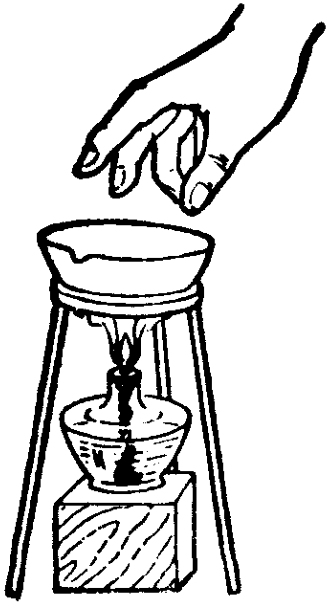
\includegraphics[width=4cm]{../pic/czhx1-xssy-27}
            \caption{\begin{minipage}[t]{4cm}
                移走正在加热\\
                的蒸发皿
            \end{minipage}}\label{fig:xssy-27}
        \end{minipage}
    \end{figure}
\end{wentihetaolun}

